\subsection{CR Alternativi: kCTF}\label{cr-alternativi-kctf}

kCTF\footnote{\label{fn:ref_4}\url{https://google.github.io/kctf/}} e\textquotesingle{}
una piattaforma sviluppata da Google, basata su \emph{Kubernetes} e
\emph{nsjail}.

\begin{quote}
\emph{Kubernetes}: e\textquotesingle{} un sistema open source per
automatizzare il deploy, scalare e gestire applicazioni
containerizzate.\footnote{\label{fn:ref_5}\url{https://kubernetes.io/}}
\end{quote}

\begin{quote}
\emph{NSJail}: ossia, NameSpace Jail, e\textquotesingle{} un tool Linux
per isolare i processi utilizzando varie feature del Kernel Linux come:
namespaces, resource limits, seccomp-bpf syscall filters.
L\textquotesingle obiettivo di NSJail e\textquotesingle{} quello di
creare un\textquotesingle ambiente sicuro e isolato per eseguire le
applicazioni. \footnote{\label{fn:ref_6}\url{https://github.com/google/nsjail/}}
\end{quote}


\begin{figure}[htbp]
  \centering
  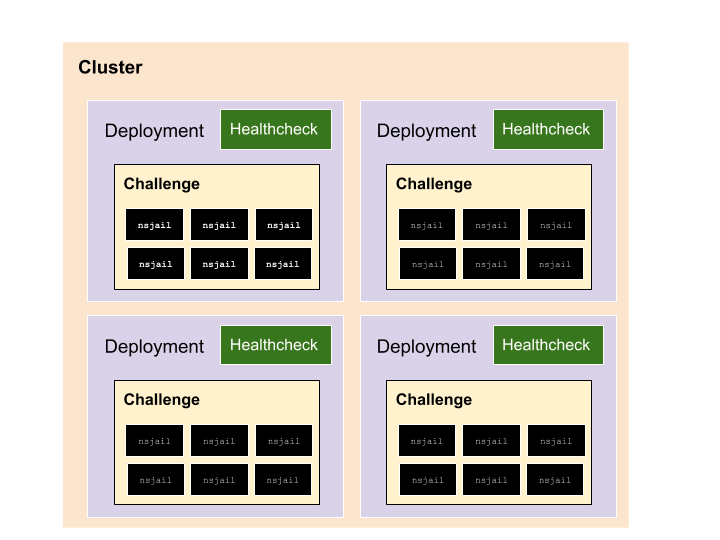
\includegraphics[width=0.85\linewidth,height=0.65\textheight,keepaspectratio]{src/images/kctf-architecture.png}
  \caption{Kctf Architecture}
  \label{fig:kctf-architecture}
\end{figure}


Facendo riferimento all\textquotesingle immagine sopra,
l\textquotesingle architettura di kCTF prevede:

\begin{itemize}
\tightlist
\item
  Un \textbf{cluster}, che contiene un\textquotesingle insieme di
  challenge
\item
  Dei \textbf{deployment}, ognuno contiene due container (o meglio, un
  Pod che instanzia 2 container):

  \begin{itemize}
  \tightlist
  \item
    un container \passthrough{\lstinline!healthcheck!}: usato per
    determinare lo stato di salute dei servizi
  \item
    un container \passthrough{\lstinline!challenge!}: contiene i servizi
    su cui lavora lo sfidante.
  \end{itemize}
\end{itemize}

\begin{quote}
\textbf{Pod}: in Kubernetes, e\textquotesingle{} la piu piccola unita
che Kubernetes puo\textquotesingle{} eseguire. Un Pod, rappresenta uno o
piu container in esecuzione su un singolo nodo.\footnote{\label{fn:ref_7}\url{https://www.k8s.guide/workloads/pods-deployments/}}
\end{quote}

\begin{quote}
\textbf{Deployment}: in Kubernetes, un deployment e\textquotesingle{} un
template che specifica come creare i container. I template guidano la
creazione di \textbf{Pods} e la gestione sicura del ciclo di vita di un
Pod, in particolare la gestione dei ReplicaSet.\footref{fn:ref_7}
\end{quote}

NSJail viene avviato su ogni container
\passthrough{\lstinline!challenge!}, ed e\textquotesingle{} configurato
per ascoltare su una porta TCP nota. Ad ogni connessione TCP in arrivo,
NSJail esegue un fork restituendo allo sfidante
un\textquotesingle ambiente separato (rispetto agli altri sfidanti) su
cui lavorare. L\textquotesingle obiettivo di questa architettura
e\textquotesingle{} di poter riutilizzare lo stesso container per piu
sfidanti.

L\textquotesingle isolamento fornito da NSJail, si ottiene combinando
varie tecniche:

\begin{itemize}
\tightlist
\item
  Creazione di nuovi namespace: l\textquotesingle ambiente fornito,
  esegue su un nuovo namespace, separando logicamente le risorse
  accessibili.
\item
  Filtraggio delle chiamate di sistema tramite
  \passthrough{\lstinline!seccomp-bpf!}: questo sottosistema permette di
  uccidere i processi nell\textquotesingle ambiente se vengono eseguite
  chiamate di sistema vietate.
\item
  Accounting e limitazione delle risorse con
  \passthrough{\lstinline!cgroup!}: questo sottosistema permette di
  monitorare e limitare le risorse utilizzabili nel nuovo ambiente.
\end{itemize}

NsJail puo\textquotesingle{} essere configurato in modo che ogni
ambiente isolato, abbia a disposizione un\textquotesingle filesystem
temporaneo che risiede in RAM, mentre il filesystem originale
e\textquotesingle{} accessibile dall\textquotesingle ambiente sandbox in
sola lettura. Questa configurazione e\textquotesingle{} necessaria
poiche altrimenti gli sfidanti modificherebbero tutti lo stesso
filesystem.

Un\textquotesingle altra configurazione di NSJail e\textquotesingle{} la
seguente: che e\textquotesingle{} ideale per le challenge di tipo
\passthrough{\lstinline!pwn!} (trovare e sfruttare vulnerabilita in file
binari):

\begin{lstlisting}
[...]
mount: [
  {
    src: "/chroot"
    dst: "/"
    is_bind: true
  },
  {
    dst: "/tmp"
    fstype: "tmpfs"
    rw: true
  },
  {
    dst: "/proc"
    fstype: "proc"
    rw: true
  },
  {
    src: "/etc/resolv.conf"
    dst: "/etc/resolv.conf"
    is_bind: true
  }
]
\end{lstlisting}

\begin{enumerate}
\def\labelenumi{\arabic{enumi}.}
\tightlist
\item
  La cartella \passthrough{\lstinline!/chroot!} che risiede nel
  container, diventa la radice nel nuovo ambiente.
\item
  Viene creato un nuovo \passthrough{\lstinline!tmpfs!}, in
  \passthrough{\lstinline!/tmp!}
\item
  Viene importata la configurazione DNS da
  \passthrough{\lstinline!/etc/resolv.conf!} dentro la nuova radice.
\end{enumerate}

Tutta via, l\textquotesingle uso di NsJail per separare gli ambienti dei
partecipanti, rende difficoltosa l\textquotesingle implementazione di
challenge in cui si vuole dare la liberta ai partecipanti di installare
pacchetti dentro al container, oppure di modificare file di
configurazione che risiedono per esempio in
\passthrough{\lstinline!/etc!} e di modificare direttamente servizi in
esecuzione sul container. \footnote{\label{fn:ref_8}\url{https://github.com/google/kctf/blob/v1/docs/security-threat-model.md}}

Queste limitazioni ci sono perche NsJail nell\textquotesingle ambiente
sandbox non fornisce una propria istanza di
\passthrough{\lstinline!systemd!} (o un qualsiasi gestore di servizi) e
neanche l\textquotesingle infrastruttura necessaria per eseguiure
comandi come \passthrough{\lstinline!apt!}.

Tale limitazione, porta ad escludere kCTF come possibile soluzione al
problema orignale esposto, suggerendo come astrazione migliore per
l\textquotesingle ambiente di un partecipante l\textquotesingle uso di
un \textbf{container} (Incus o Docker), piuttosto che una sandbox
generata da NsJail.

TODO: \textbf{Problemi}:

\begin{itemize}
\tightlist
\item
  in nsjail il filesystem e\textquotesingle{} disponibile in sola
  lettura. Comandi come \passthrough{\lstinline!apt!} e modifiche
  diretta a \passthrough{\lstinline!/etc!} non funzionano.
\item
  se la connessione TCP cade allora tutto il lavoro che risiede in RAM
  e\textquotesingle{} perso
\item
  in nsjail, l\textquotesingle applicazione di filtri seccomp potrebbero
  impedire l\textquotesingle esecuzione di alcune chiamate di sistema.
\item
  kCFT usa Kubernetes introducendo costi e complessita.
\end{itemize}
